\documentclass[journal]{IEEEtran}
\usepackage{cite}
\usepackage[pdftex]{graphicx}
\graphicspath{{./images/}}

% *** MATH PACKAGES ***
\usepackage[cmex10]{amsmath}
% *** SPECIALIZED LIST PACKAGES ***
\usepackage{algorithmic}
% *** ALIGNMENT PACKAGES ***
\usepackage{array}
%\usepackage{mdwmath}
%\usepackage{mdwtab}
%\usepackage{eqparbox}
% *** TIKZ ***
% Required packages and libraries
\usepackage {tikz}
\usetikzlibrary {patterns}
\usepackage{tkz-euclide}
% \usetkzobj{all}


% \usepackage{tikzpicture} %preamble
% *** SUBFIGURE PACKAGES ***
%\usepackage[tight,footnotesize]{subfigure}
%\usepackage[caption=false]{caption}
%\usepackage[font=footnotesize]{subfig}
% *** FLOAT PACKAGES ***
%\usepackage{fixltx2e}
\usepackage{stfloats}
% *** PDF, URL AND HYPERLINK PACKAGES ***
%\usepackage{url}
\usepackage{hyperref}
% \url{my_url_here}.
% *** Do not adjust lengths that control margins, column widths, etc. ***
% *** Do not use packages that alter fonts (such as pslatex).         ***

% correct bad hyphenation here
\hyphenation{op-tical net-works semi-conduc-tor}

\begin{document}
%
% paper title
% can use linebreaks \\ within to get better formatting as desired
\title{Double Inverted Pendulum: \\
Stable Control via Feedback Linearization with
Python Simulation and Analysis}
\author{Bardia~Mojra}
% make the title area
\maketitle

\begin{abstract}
Stable control of the Double Inverted Pendulum (DIP) is a classic hard problem in
control systems. The system is highly nonlinear and sensitive to
the initial conditions. This article focuses on the derivation of
\emph{equations of motion} and \emph{feedback linearization} method which,
were used to develop a symbolic representation of the system. We show that the
system characteristic matrix is positive definite and is invertible as required
by \emph{Lyapunov's direct method}. Using MATLAB
Control Toolbox, we solve the continuous \emph{Lyapunov Control Function} to
obtain the \emph{linear quadratic regulator} (LQR) solution which is considered
to be unique, stable, and optimal. To enhance this case study,
an end-to-end software suite is developed in Python to simulate and animate the system. Moreover, a series of experiments are designed and performed to study 1) effects of variations in model
parameters (i.e. masses, pendulum lengths, and friction).
2) To quantify system behavior and stability at different initial condition, given tuned and
untuned control parameters. 3) And to investage and discover some evidence of
the chaotic nature of the system, as well as capturing it. The software suite
developed for this project will be made available to public to MIT license at \href{https://github.com/BardiaMojra/dip}{github.com/BardiaMojra/dip}.

\end{abstract}

% \IEEEpeerreviewmaketitle


\section{Introduction}
This is the intro\\




% keep this at the bottom of the page
% \hfill {\today}\\
% \hfill




\subsection{Related Work}
This is related \\

\subsection{Objectives}
The objective of this article is to present a concise, intuitive and transferable
the solution to a classical optimal control problem.
Our objective is to model the plant using Lagrange's equations of motion,
derive state dynamics, obtain a generalized cost function, and to optimally
control the double pendulum by reaching a stable configuration in the upright
position while given minim-energy control input to the system.\\
Also --- testing\\
Also ---\\

\subsection{Article Structure}



\section{Estimation Formulation}
There are many benefits to using the \emph{state space} framework, notably that
is well generalized and conveniently implemented on modern computers.

\subsection{System Setup}
Consider a resting cart on a flat rigid surface along the x-axis, on top of
which are stacked two inverted pendulums, figure 01. The pendulums resemble a
robotic arm but rather without a motor or external torque input. At the end of
each pendulum is assumed to be a point-mass, \(m_1\), \(m_2\). Each pendulum
moves freely and independently and is connected by lengths \(l_1\) and \(l_2\)
from their joints, \(q_1\) and \(q_2\) to their point-masses, \(m_1\),
\(m_2\). The mass of the cart is considered point-mass as well and is denoted
by \(m_c\) with its position \(q_c\) along the x-axis. \(\theta_1\) and
\(\theta_2\) denote angular deviations from upright position for \(q_1\) and
\(q_2\), respectively.

% add figure here -- system setup DIP

\begin{figure}[!t]
    \centering
    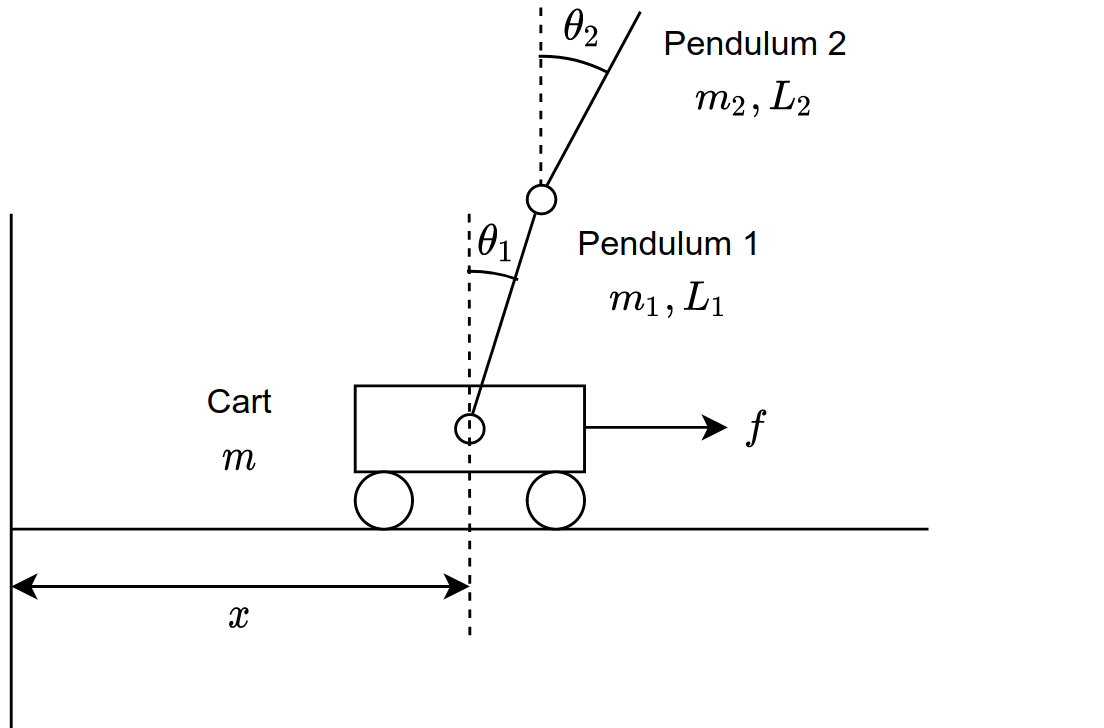
\includegraphics[width=2.5in]{fig01_cart001.png}
    \caption{Physical System}
    \label{fig_sim}
\end{figure}

% \begin{tikzpicture} [thick]

%     % Angle of Pendulum
%     \newcommand{\anga}{26.5}
%     \newcommand{\angb}{-20}

%     % grid
%     \draw[step=.5, lightgray] (-2,0) grid (2, 6);
%     % ground
%     \draw [brown!80!red] (-2,0) -- (2,0);
%     \fill [pattern = crosshatch dots,
%         pattern color = brown!80!red] (-2,0) rectangle (2,-.2);

%     % cart and DIP scope
%     \begin{scope} [draw = orange,
%         fill = orange!20,
%         dot/.style = {orange, radius = .025}]

%     % point coords
%     \coordinate (q1) at (0,1.5);
%     \coordinate (m1) at (1, 3.5);
%     \coordinate (m2) at (-.5, 5.5); % [label=left:$m_2$]


%     % rod 1
%     \filldraw [rotate around = {-\anga:(q1)}] (.09,1.5) --
%         node [midway, right] {$l_1$}
%         % node [very near end, right] {$m_1$}
%         +(0,2.15) arc (0:180:.09)
%         coordinate [pos = .5] (T) -- (-.09,1.5);
%     % rod 2
%     \filldraw [rotate around = {0:(m2)}] (m1)+(-.09,1.5) --
%         node [midway, left] {$l_2$}
%         +(0,2.15) arc (0:180:.09)
%         coordinate [pos = .5] (C) -- (m1) + (.09, 1.5);

%     % masses
%     % \shade [ball color=blue] (m1) circle [radius=.2cm];
%     % \shade [ball color=blue] (m2) circle [radius=.2cm];

%     % wheels
%     \filldraw (-.65,.15) circle (.15);
%     \fill [dot] (-.65,.15) circle;
%     \filldraw (.65,.15) circle (.15);
%     \fill [dot] (.65,.15) circle;


%     \filldraw (-1,1.5) -- coordinate [pos = .5] (F)
%         (-1,.3) -- node [above = .3cm] {$m_c$}
%         (1,.3) -- (1,1.5)
%         coordinate (X) -- (.1,1.5)
%         arc (0:180:.1) -- (-1.014,1.5);

%     \fill [dot] (0,1.52) circle;
%     \end{scope}

%     % lines and angles
%     \begin{scope} [thin, orange!50!black]
%         \draw (T) -- (0,1.52) coordinate (P);
%         \draw [dashed] (P) + (0,0) -- +(0,1.25);
%         \draw (P) + (0,.5) arc (90:90-\anga:.5) node [black, midway, above] {$\theta_1$};
%         \draw (0, 3) node [black, midway, above = 1.1cm] {$q_1$};
%     \end{scope}

%     % forces
%     \draw [stealth-] (F) -- node [above] {$u$} + (-1,0);
%     % \draw [-stealth] (X) |- node [very near end, above right] {$x$} + (1,.3);

%     % xy axis
%     \draw [-stealth] (-2,2) -- (-2,3) node[midway, right] {$y$};
%     \draw [-stealth] (-2,2) -- (-1,2) node[midway, above] {$x$};

% \end{tikzpicture}

\subsection{State Definition}
Suppose we have a continuous-time, nonlinear system presented in state space
form.
% ss form

\begin{equation}
    % \label{eq:6}
    \dot{x} = f(x,u),
\end{equation}
\begin{equation}
% \label{eq:7}
    y = h(x).
\end{equation}

whats f - prediction model
whats h - obs model
omit obs noise, it requires EKF??

Our goal is to stabilize the described highly nonlinear system in the upright
configuration

\subsection{Noise and Friction}
% paper

\subsection{Global Coordinate Frame}
We need to form a homogenous configuration space to present state variables
\(q, \theta_1, \theta_2\) by forming a global coordinate frame with \(x(t=0)\)
as the origin.
\begin{equation}
    \begin{split}
    % \label{eq:6}
    q_c = \begin{bmatrix}
    q \\
    0 \\
    \end{bmatrix}, ~~
    q_1 = \begin{bmatrix}
    q + l_1 \sin \theta_1 \\
    l_1 \cos \theta_1 \\
    \end{bmatrix}, \\
    % \label{eq:6}
    q_2 = \begin{bmatrix}
    q + l_1 \sin \theta_1 + l_2 \sin \theta_2 \\
    l_1 \cos \theta_1 + l_2 \cos \theta_2 \\
\end{bmatrix},
\end{split}
\end{equation}
\noindent
We denote position of point-masses for \(m_c\), \(m_1\), and
\(m_2\) by \(q_c, q_1, q_2 \in R^2\) on the x-y plane.
We seek to define our system in terms of these state variables. Thus, we define
state variable vector \(q(t)\) as
\begin{equation}
q = [q_c, q_1, q_2]^{T}
\end{equation}
In later section, we formally rewrite state variable definitions independent of
time \(t\) via a linearization process. For simpler representation, we
denote state variable vector as \(q:=q(t)\).

\subsection{Other Considerations}
Noise and Friction modeling, process noise versus observation noise.

\section{Model Derivation}
% steps



\subsection{Equations of Motion}
As it is laid out in \emph{Lagrangian mechanics}; first we must obtain the Lagrangian
of the physical model, \(\mathcal{L}= K -P\). \(K\) and \(P\) represent the
\emph{kinetic} and \emph{potential} energies of the system. \(K\) is the total
kinetic energy from all three masses and in later sections, we will discuss
transforming \emph{Lagrangian mechanics} to \emph{Hamiltonian mechanics} by
replacing velocities with \emph{momenta}. Here, we define K as
\begin{equation}
    K = \frac{1}{2} m v^2 =~ \frac{1}{2} {m_c\|\dot{q_c}\|^2 + m_1\|\dot{q_1}\|^2 + m_2\|\dot{q_2}\|^2}.
\end{equation}

P denotes the overall potential energy of the system; but since the cart rolls
flat along the x axis, it is inherently incapable of storing energy so we discard
it. P is obtained by
\begin{equation}
    P = g \left[ m_1 l_1 \cos \theta_1 + m_2 (l_1 \cos \theta_1 + l_2 cos \theta_2) \right]
\end{equation}
Where \(g \in R\) denotes gravitational acceleration.
Next, we envoke the \emph{Euler-Lagrange} equation to write the following ODE system
whose solution is the position and velocity configuration vector of the cart
and masses on the x-y plane, given the final time, previous state, system
dynamics, control input and disturbances.
\begin{equation}
    y(t) = f(t,q,\dot{q},u,\omega)
\end{equation}
\emph{The Lagrange Equations of Motions} are defined as
\begin{equation}
    Q = \frac{\partial\mathcal{L}}{\partial f_{i}} - \frac{d}{dt} \left( \frac{\partial \mathcal{L}}{\partial f_{i}}\right).
\end{equation}
Where \(Q\) represents the vector of sum of external forces acting on the plan.
\begin{equation}
    \mathcal{L} = \mathcal{L}(t, q, \dot{q})
\end{equation}
\begin{equation}
\begin{cases}
\begin{array}{rcl}
    u + \omega_1 -d_1 \dot{q} &=& \frac{d}{dt} \{\frac{\partial\mathcal{L}}{\partial\dot{q}}\}-\{\frac{\partial\mathcal{L}}{\partial q}\}\\
    \omega_2 -d_2 \dot{\theta_1} &=& \frac{d}{dt} \{\frac{\partial\mathcal{L}}{\partial\dot{\theta_1}}\}-\{\frac{\partial\mathcal{L}}{\partial \theta_1}\}\\
    \omega_3 -d_3 \dot{\theta_2} &=& \frac{d}{dt} \{\frac{\partial\mathcal{L}}{\partial\dot{\theta_2}}\}-\{\frac{\partial\mathcal{L}}{\partial \theta_2}\}\\
    \end{array}
\end{cases}
\end{equation}

So far our derivation has made our expressions more complicated but these steps are
neccessary for capturing the full dynamical characteristics of the system. In the
following section, we derive the continuous-time nonlinear model of described
system. Moreover in \emph{Optimal Control} section, we briefly explain how one
could derive \emph{the general optimal control solution} for a \emph{positive
definite and semidefinite energy system} with known characteristic parameters.
Moreover, we intuitively explain and reference why we could consider the solution
space to such a ODE as \emph{smooth manifold} that maps current and future state
through recursion and its energy state decays towards a local minima.


\subsection{Continues-Time, Nonlinear Model}
We used MATLAB Symbolic Math Toolbox to derive the resultant ODE. Obtaining
symbolic or implicit expressions of our ODE will allow us to analytically derive
to the optimal solution.
\begin{equation}
\text{\scriptsize $
% \begin{cases}
\begin{array}{rcl}
        u + \omega_1 -d_1 \dot{q} &=& (m_c+m_1+m_2)\ddot{q}+l_1(m_1+m_2)\ddot{\theta_1} \cos \theta_1\\
        & & + m_2 l_2 \ddot{\theta_2} \cos \theta_2 - l_1 (m_1+m_2) \dot{\theta_1}^2 \sin \theta_1 \\
        & & - m_2 l_2 \dot{\theta_2}^2 \sin \theta_2\\
        \omega_2 -d_2 \dot{\theta_1} &=& l_1 (m_1+m_2) \ddot(q) \cos \theta_1
        +l_1^2 (m_1+m_2) \ddot{\theta_1}\\
        & & +l_1 l_2 m_2 \ddot{\theta_2} \cos (\theta_1 - \theta_2)+ l_1 l_2 m_2 \dot{\theta_2}^2 \sin(\theta_1 - \theta_2) \\
        & & - g(m_1+m_2) l_1 \sin \theta_1 \\
        \omega_3 -d_3 \dot{\theta_2} &=& l_2 m_2 \ddot{q} \cos \theta_2
        + l_1 l_2 m_2 \ddot{\theta_1} \cos (\theta_1 -\theta_2)
        + l_2^2 m_2 \ddot{\theta_2}\\
        & & -l_1 l_2 m_2 \dot{\theta_1}^2 \sin (\theta_1 - \theta_2)
        - l_2 m_2 g \sin \theta_2\\
    \end{array}
% \end{cases}
$}
\end{equation}

\subsection{Optimal Control}
% define
% in other words
% so we do this

\subsection{Linearization}
First, we rewrite the equations of motion into matrix form to batch acceleration,
velocity, and position terms into separate matrices. A second order representation
of the physical system is sufficient to provide an accurate enough estimate,
per \emph{Taylor Series Linearization} method. This is an important step as
identifying system dynamics lies at the heart of \emph{Optimal Control}.
\begin{equation}
D(q) \ddot{q} + C(q, \dot{q}) \dot{q} + G(q) = Hu
\end{equation}
where matrix functions \(D(q) \ddot{q} + C(q, \dot{q}) \dot{q} + G(q)\)
represent systems dynamics with respect to time,
current state and previous state. Time variable \(t\) is omitted to simplify
notation. The system energy state (left hand side of
above EOM) is presented in relation to external forces \(Hu\) acting on the
system. Vector \(u \in R^1\) represents external input forces vector and matrix
\(H\) represents its relationship with state variable functions. Matrix
functions \(D(q),~C(q, \dot{q}),~G(q)\) and vector H are define as

\begin{equation}
% \text{\scriptsize $
% \begin{cases}
% \begin{array}{rcl}
    D(q) = \begin{pmatrix}

    \end{pmatrix}
% \end{array}
% \end{cases}
% $}
\end{equation}


Before we perform linearization, we need to rewrite the EOM in the following
matrix form to obtain the final ODE. By doing so, we rewrite state dynamics as
a function of derivative terms instead of time (\emph{isomorphism}). Per \emph{Lyapunov
Control Function theory} (LCF) for autonomous dynamical systems and
\emph{LaSalle's}, we can assume there exists at least one
\emph{Optimal Control Trajectory} or \emph{Hamiltonian Flow} for any acceptable
initial conditon if the LCF is \emph{positive definite} or \emph{positive
semi-definite}. Moreover, the energy function must be \emph{isomorphic} and
\emph{symmetric} in order to form \emph{stable} control trajectory.

\begin{equation}
M(q)\dot{q} = A(q)q + Bu
\end{equation}

Where \emph{positive definite} or \emph{positive semi-definite} constraints are
evaluated by computing the determinant of \(M\).
\begin{equation}
det(M) > 0;~ \forall q
\end{equation}
Such that, the final ODE can be written as
\begin{equation}
    \dot{q} = M(q)^{-1}(A(q)q + Bu)
\end{equation}
To make remove the time index and make the ODE fully \emph{isomorphic}, we
define a new variable state vector as
\begin{equation}
    x:=
    \begin{bmatrix}
        y \\
        \dot{y}\\
    \end{bmatrix}
\end{equation}

L(x, u) =
 x T
 Qx + uT Ru


we
\subsection{Discrete, Linear Model}
\begin{equation}
\begin{array}{rcl}
    x &=& Ax + Bu \\
    y &=& \dot{x} \\
\end{array}
\end{equation}

where A and B are defined as
\begin{equation}
    A =
\begin{bmatrix}
        0 & I \\
        D^{-1} \frac{\partial G}{\partial q} & 0 \\
\end{bmatrix}
\end{equation}

\begin{equation}
    B =
\begin{bmatrix}
    0 \\
    D^{-1} H\\
    \end{bmatrix}
    \end{equation}

\subsection{General Time-Invariant Cost Function and Linear Quadratic Regulator SolutionLQR}
So far, we have modelled, linearized and discretized our system using state
space general form. In the process, we systematically reduced the solution space
complexity by replacing time \(t\) and velocity dimension as linear products of
current and previous states. This allows us to analytically derive a general
form optimal solution. But before we reach that step, we need to define a
general \emph{Cost Function} \(J\) that only depends on absolute minimal parameters,
which we will later optimize to arrive to a \emph{minimal surface}. Quadratic
performance index \(J \) is
defined as [see page 24 of Optimal control - now we can optimize similar to static cases]
\begin{equation}
J(x,u) = \frac{1}{2}x^{T}Q x + \frac{1}{2}u^{T}Ru
\end{equation}
whose solution is the minimal cost or minimun-energy input required for the
system to reach local minima, for any given initial state. Next, we minimize \(J\)
which will yield the state feedback weight vector \(K\) and is obtained by
recursively solving the dynamic \emph{Riccati} equation.
It is important to note that calculation of Quadratic losses are carries out by
performing dot product of state vector with its transpose and energy magnitude.


\section{Simulations and Results}
% Python simulation
% https://www.do-mpc.com/en/v4.1.0/example_gallery/DIP.html1




% Note that IEEE typically puts floats only at the top, even when this
% results in a large percentage of a column being occupied by floats.


% An example of a double column floating figure using two subfigures.
% (The subfig.sty package must be loaded for this to work.)
% The subfigure \label commands are set within each subfloat command, the
% \label for the overall figure must come after \caption.
% \hfil must be used as a separator to get equal spacing.
% The subfigure.sty package works much the same way, except \subfigure is
% used instead of \subfloat.
%
% \begin{figure*}[!t]
% \centerline{\subfloat[Case I]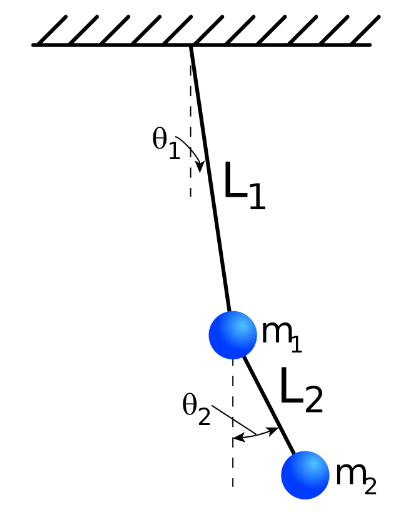
\includegraphics[width=2.5in]{dpend.png}%
% \label{fig_first_case}}
% \hfil
% \subfloat[Case II]{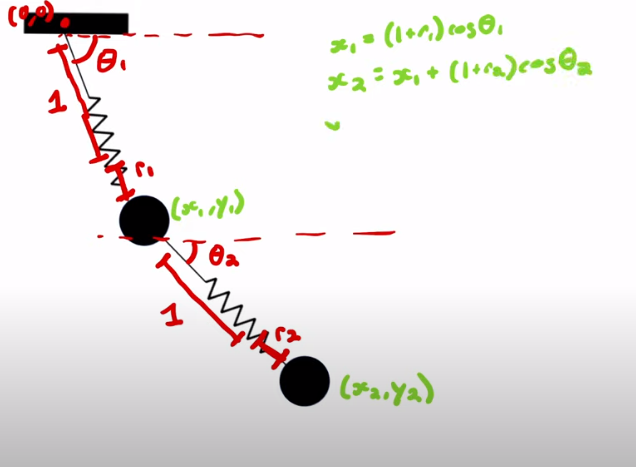
\includegraphics[width=2.5in]{dpend_sprg.png}%
% \label{fig_second_case}}}
% \caption{Simulation results}
% \label{fig_sim}
% \end{figure*}
%
% Note that often IEEE papers with subfigures do not employ subfigure
% captions (using the optional argument to \subfloat), but instead will
% reference/describe all of them (a), (b), etc., within the main caption.


% An example of a floating table. Note that, for IEEE style tables, the
% \caption command should come BEFORE the table. Table text will default to
% \footnotesize as IEEE normally uses this smaller font for tables.
% The \label must come after \caption as always.
%
%\begin{table}[!t]
%% increase table row spacing, adjust to taste
%\renewcommand{\arraystretch}{1.3}
% if using array.sty, it might be a good idea to tweak the value of
% \extrarowheight as needed to properly center the text within the cells
%\caption{An Example of a Table}
%\label{table_example}
%\centering
%% Some packages, such as MDW tools, offer better commands for making tables
%% than the plain LaTeX2e tabular which is used here.
%\begin{tabular}{|c||c|}
%\hline
%One & Two\\
%\hline
%Three & Four\\
%\hline
%\end{tabular}
%\end{table}


% Note that IEEE does not put floats in the very first column - or typically
% anywhere on the first page for that matter. Also, in-text middle ("here")
% positioning is not used. Most IEEE journals use top floats exclusively.
% Note that, LaTeX2e, unlike IEEE journals, places footnotes above bottom
% floats. This can be corrected via the \fnbelowfloat command of the
% stfloats package.



\section{Conclusion}
The conclusion goes here.







% \appendices
% \section{Proof of the First Zonklar Equation}
% Appendix one text goes here.

% you can choose not to have a title for an appendix
% if you want by leaving the argument blank
% \section{Appx B title}
% Appendix two text goes here.


% use section* for acknowledgement
\section*{Acknowledgment}
The authors would like to thank...


% Can use something like this to put references on a page
% by themselves when using endfloat and the captionsoff option.
% \ifCLASSOPTIONcaptionsoff
%   \newpage
% \fi

% trigger a \newpage just before the given reference
% number - used to balance the columns on the last page
% adjust value as needed - may need to be readjusted if
% the document is modified later
%\IEEEtriggeratref{8}
% The "triggered" command can be changed if desired:
%\IEEEtriggercmd{\enlargethispage{-5in}}

% references section

% can use a bibliography generated by BibTeX as a .bbl file
% BibTeX documentation can be easily obtained at:
% http://www.ctan.org/tex-archive/biblio/bibtex/contrib/doc/
% The IEEEtran BibTeX style support page is at:
% http://www.michaelshell.org/tex/ieeetran/bibtex/
%\bibliographystyle{IEEEtran}
% argument is your BibTeX string definitions and bibliography database(s)
%\bibliography{IEEEabrv,../bib/paper}
%
% <OR> manually copy in the resultant .bbl file
% set second argument of \begin to the number of references
% (used to reserve space for the reference number labels box)
\begin{thebibliography}{1}

\bibitem{IEEEhowto:kopka}
H.~Kopka and P.~W. Daly, \emph{A Guide to \LaTeX}, 3rd~ed.\hskip 1em plus
  0.5em minus 0.4em\relax Harlow, England: Addison-Wesley, 1999.

\end{thebibliography}

% biography section
%
% If you have an EPS/PDF photo (graphicx package needed) extra braces are
% needed around the contents of the optional argument to biography to prevent
% the LaTeX parser from getting confused when it sees the complicated
% \includegraphics command within an optional argument. (You could create
% your own custom macro containing the \includegraphics command to make things
% simpler here.)
%\begin{biography}[{\includegraphics[width=1in,height=1.25in,clip,keepaspectratio]{mshell}}]{Michael Shell}
% or if you just want to reserve a space for a photo:

% \begin{IEEEbiography}{Michael Shell}
% Biography text here.
% \end{IEEEbiography}

% % if you will not have a photo at all:
% \begin{IEEEbiographynophoto}{John Doe}
% Biography text here.
% \end{IEEEbiographynophoto}

% insert where needed to balance the two columns on the last page with
% biographies
%\newpage


% You can push biographies down or up by placing
% a \vfill before or after them. The appropriate
% use of \vfill depends on what kind of text is
% on the last page and whether or not the columns
% are being equalized.

%\vfill

% Can be used to pull up biographies so that the bottom of the last one
% is flush with the other column.
%\enlargethispage{-5in}



% that's all folks
\end{document}
